\begin{figure}[h]
  \centering

  % \caption{An old painting of Isaac Newton writing the theory of gravity in the language of probability and questioning the role of models in the world. Made by $\text{DALL}\cdot\text{E }2$.}
  \includegraphics[width=.75\textwidth]{figures/chapter01/DALLE2_prof_student.png}
  \label{}
\end{figure}

\vfill

{
\textit{\justify
   First, we guess a law. Then we compute the consequences of the guess and then we compare the computation results to nature to see if it works.
  If it disagrees with experiment, it's wrong. In that simple statement is the key to science.
   It doesn't make any difference how beautiful your guess is, it doesn't matter how smart you are who made the guess. If it disagrees with experiment, it's wrong. That's all there is to it.}

  \par\bigskip
  \raggedleft\MakeUppercase{Richard Feynman}\par%
}

\vspace{4em}
%
% {\centering
% \parbox{\textwidth}{%
%   \raggedright{%\itshape%
%
%   The physical laws, in their observable consequences, have a finite limit of precision.\par\bigskip
%   }
%   \raggedleft\MakeUppercase{Kurt G{\"o}del}\par%
% }}
%
% \vspace{4em}
% {\centering
% \parbox{\textwidth}{%
%   \raggedright{%\itshape%
%
%   All generalizations, with the possible exception of this one, are false.\par\bigskip
%   }
%   \raggedleft\MakeUppercase{Kurt G{\"o}del}\par%
% }}

\vfill




\chapter{Introduction}\label{ch:introduction}
\begin{figure}[!h]
  \centering
  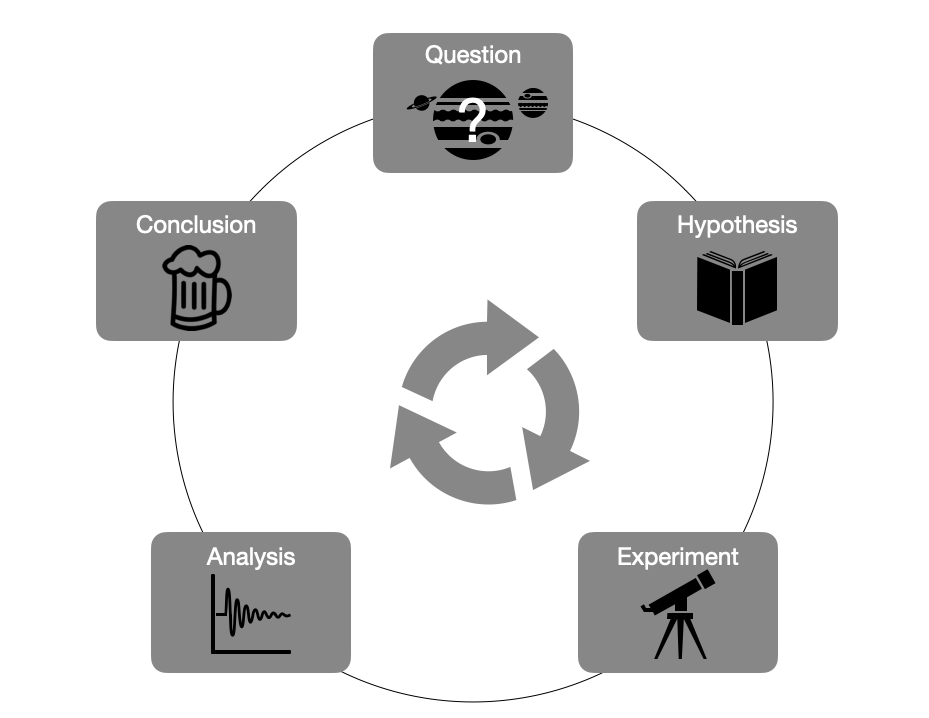
\includegraphics[width=.75\textwidth]{figures/chapter01/trapist_disco.png}
  \caption{
  Illustration of the scientific inquiry as a simplified 5-step process. The pictograms sketch a cartoon of the TRAPPIST-1 planetary system discovery made by astronomers from Li{\`e}ge University in 2016 \citep{gillon2017seven}. Scientists shall first formulate a \textit{research question} and a set of reasonable \textit{hypotheses}, together they define a class of hypothetical models of the world. In order to answer their question, scientists gather data from \textit{experiments} and analyze them in the context of their modelling assumptions. Checking the consistency of different hypothetical models allows them \textit{to provide an answer} to their initial question up to a certain degree of certainty.}
  \label{fig:ch01:scientific_method}
\end{figure}

Ever since the beginning of their existence, humans have always been curious to understand the world's complexity. This is not only true at the individual level, as we keep building and improving our knowledge over our lifespan, but also at the level of humankind, where knowledge has never really stopped rising since the beginning of civilisation. As an objectification of our curiosity, science aims to ground the construction of this common knowledge on rationality. In particular, the modern scientific method arguably relies on five pillars, as depicted in \Cref{fig:ch01:scientific_method}, which ensure discoveries are made out of rigour and based on current scientific knowledge. Although the scientific method can answer questions in the context of a specified model of the world as stated by the hypotheses, the more fundamental goal of science is to refine these models by criticising their ability to predict the real world. In this context, this thesis aims to explore and contribute to modern techniques for building or refining models of the world.

Classically, scientists or engineers use their domain expertise to build incrementally complex models and improve their faithfulness to reality. The scientific method is then applied to validate or reject the new class of models. This strategy has not only led to today's state of science but also to the uttermost engineering accomplishments of modern times. In engineering, these successes impact our daily life, such as by enabling nuclear electricity - as predicted by special relativity - or allowing one to read this manuscript on a smart tablet - thanks to Maxwell equations' implications on the design of modern computers. More abstract but arguably as impactful on our vision of the universe, the classical model refinement strategy led to all modern scientific breakthroughs. As an example, these models allow astronomers to observe the furthest human-known objects, thanks to general relativity and gravitational lensing and enable the indirect observations of black holes thanks to gravitational waves theory.

Despite these numerous achievements, machine learning has recently challenged the classical modelling approach. Where humans fall short of finding patterns in a large amount of data and build arbitrarily complex models by themselves, machines can automatically perform these tasks day and night. The paradigm shift from hand-crafted to automated modelling happens in a world where the most ambitious scientific experiments generate petabytes ($10^{15}$) of data per second \citep{noauthor_cern_nodate}. On the one hand, while the computing capacity continuously increases, the human brain is not better wired to apprehend vast amounts of data than it was when Galileo Galilei set the basis of modern science 400 years ago. On the other hand, deep learning has recently proven its ability to build accurate generative models that outperform the ones designed out of human expertise. This is, for example, true in the context of voice synthesis \citep{van_den_oord_wavenet_2016}, text-translation \citep{brown2020language, devlin2018bert}, chatbots \citep{alayrac2022flamingo}, or even text-to-image synthesis \citep{ramesh2022hierarchical, saharia2022photorealistic}, to cite a few. Among these models, some impersonates human artists. For instance, \Cref{fig:dalle-mini} shows images produced by a small version of $\text{DALL}\cdot\text{E}$ 2, a machine learning model capable of generating images from text descriptions. Under these circumstances, the paradigm shift seems natural, even in a scientific context.


\begin{figure}
  \centering
  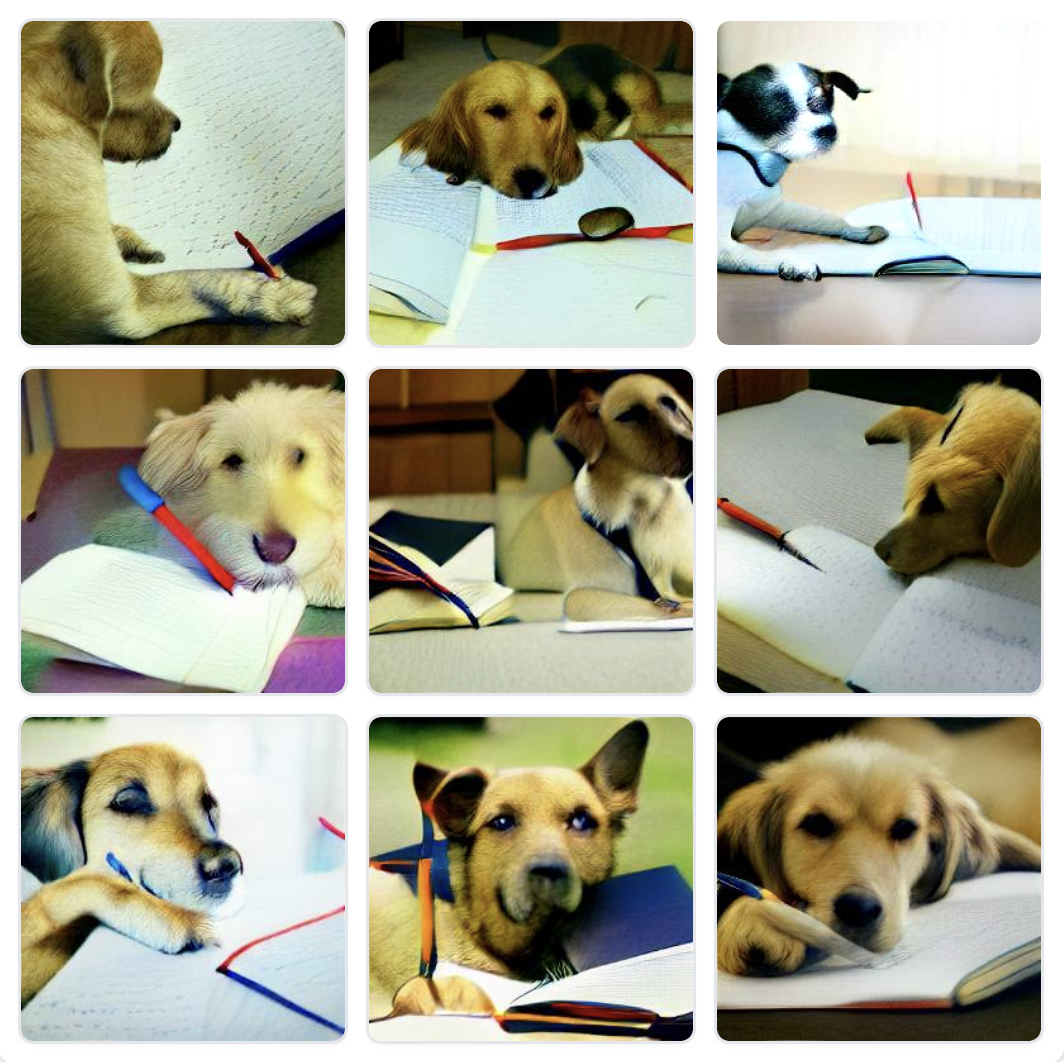
\includegraphics[width=.7\textwidth]{figures/chapter01/dog_phd_thesis.jpeg}
  \caption{\textit{A dog writing a PhD thesis}, generated by $\text{DALL}\cdot\text{E}$ mini~\citep{Dayma_DALL_E_Mini_2021}.}
  \label{fig:dalle-mini}
\end{figure}

% Of particular interest to this thesis are probabilistic models that account for the uncertainty going with modelling assumptions and the partial observability of model's variables.
Machine learning has revolutionised the way we build models over the past decades. Yet, modelling \textit{uncertainty} with machine learning models is still a very active research field. Models that account for uncertainty are called \textit{probabilistic models} and describe non-deterministic relationships between the quantities of interest. When it comes to machine learning, these descriptions often take the form of a \textit{generative model} that synthesise realisations of the phenomenon of interest. For example, $\text{DALL}\cdot\text{E}$ 2 is what we call a \textit{deep generative model}; it parameterises a generative process from textual description to plausible images with deep neural networks.

Despite some great successes, automating probabilistic model discovery remains an active research area. One of the great features of ML algorithms, their genericity, is also an important flaw. The weak assumptions behind ML models contrast with the classical modelling approach, which is grounded on a deep understanding of the phenomenon of interest. The term \textit{inductive bias} refers to all the weak assumptions made by the machine learning algorithm, such as continuity or invariance. Together with large amounts of data, the inductive bias of current ML algorithms suffices for some modelling tasks such as image or audio synthesis. However, this approach fails in scarce data settings or on data modality for which the inductive bias of existing learning algorithms is not appropriate. In contrast to the classical modelling approach, ML algorithms do not exploit effectively existing prior knowledge. Moreover, existing algorithms exhibit other limitations, such as training instabilities and lack of expressivity, to cite a few.

% A paragraph on the progress in deep generative models over the last years and the history behind it, from deep belief networks to diffusion models. Most of the progress
% made for images and text. A bit for sound as well. These are signals for which we can easily gather tons of data. And this showcase that deep models can learn a useful representation from this large dataset. But this is far from being able to say that automated modelling can challenge classical modelling in all settings. In particular, there are two classes of complication that come jointly with all current approaches: 1) All current generative models require are very difficult to train and require expertise of these models, the tricks required can vary with the data modalities and so there are still huge area for improvement to simplify the broad utilization of these algorithms. 2) These algorithms only rely on architectural inductive bias, which might be sufficient for images, text and sounds that are well suited for convolutions and attentions but they are not made to use other kind of prior knowledge we may have of the process of interest, this is a piece that miss to overpass the classical approach on many important modelling tasks.

% Sounds, text, images, all these successes correspond to modalities for which data are broadly available. This hints that deep generative models can process and create valuable representations of large datasets. It is tough to quantify if these models understand the structure of the data or if they are intelligent copycats. For example, it is not always easy to ensure that these models do not collapse to a subset of the modes present in the data. Depending on the aim of the model, mode collapse can be problematic, e.g. if we want to handle inherent stochasticity observed in the data. In addition, recent works argue that these large models do overfit the training data \citep{overfit_dalle, gpt3}.
% This makes sense as nothing helps a neural network knowing something it has not seen during training. This may preclude the application of deep generative models in contexts where data are scarcer or if we aim for a model with a profound understanding of the phenomenon it is trained to represent. \textcolor{red}{Upgrade this paragraph!!}
% % A partial solution to this problem would be to allow these models to use efficiently the prior knowledge we can have of the modeled process, this is maybe fine when the goal is to do image synthesis but is not when we need a model that satisfies the laws of physics.
% Paragraph on the challenges faced by deep generative models: Trainign difficulty, generalization, consistency with law of physics, interpretability.

\begin{side_note}{Explicit vs. implicit models}
  In general, accurate modelling requires accounting for uncertainty. Modelling uncertainty is essential as, by definition, models are simplified representations of reality; they cannot explicitly represent all possible sources of perturbations deterministically.
  For instance, we determine the precision of any sensor by fitting a model that accounts stochastically for internal and external perturbations that may arise in practical settings such as temperature, humidity or pressure variations. This inherent stochasticity exists both for small models that are simplistic representations and for larger models that are a combination of smaller stochastic models. These models describe the stochastic relationship between observations $\mathbf{x}$ provided the models' parameters $\mathbf{\theta}$. %The complexity of the models eventually depends on the granularity of the various aggressors modelled.

  While simple models lead to tractable likelihood functions $p(\mathbf{x}|\mathbf{\theta})$, larger models are computer programs for which the likelihood is usually intractable because of the multiple sources of randomness. We use the terms \textit{explicit} and \textit{implicit} to distinguish between models that provide direct access to the likelihood function and those that do not. We use the same terms for deep probabilistic models that provide access to the likelihood or solely to the generative process.
\end{side_note}
\section{Research question}

Motivated by this paradigm shift and the remaining challenges in deep probabilistic modelling, this thesis contributes to answering the following research question: \textbf{how can we improve the automatic discovery of probabilistic models with deep learning algorithms?}

In pursuing this objective, we explore several directions that study and improve upon various aspects of deep probabilistic models. In particular, we distinguish between data-driven models and hybrid models. On the one hand, the performance of data-driven models mainly depends on the learning algorithm's inductive bias and the availability of representative data. These algorithms are well suited to modelling tasks for which we do not have strong domain knowledge but access to many representative data. On the other hand, hybrid models are informed by solid prior knowledge, e.g. independencies or partial understanding of the underlying physics. Hybrid modelling allows the combination of domain knowledge with data and is thus better equipped against small or less-representative datasets. We argue that contributions to both modelling strategies are complementary and will improve the range of application of deep probabilistic models.
% A word somewhere that scientific models are usually probabilistic generative models because good models require modelling uncertainty coming from unmodeled phenomenon or phenomenon
% that are only modeled up to a certain level of stochasticity. Introduced the concept of explicit generative vs implicit generative models

% Paragraph arguing that we still need to work on deep generative models as they are not perfect yet.


% Even granted with perfect optimization procedures and universal generative models, the problem would not be solved. To fight the curse of dimensionality
% we need strong inductive bias. But more than the curse of dimensionality we also often requires these models to not stupidly fall as soon as they are required to
% act in an environment slightly different from the training configuration. We want these models to be able to built on current knowledge. It may also be important that these Models
% have a level of interpretability for humans especially if we want to use them in a scientific context. The second part of this thesis study this equally important aspect.


\section{Outline and structure}

Before diving into the core contributions of this thesis, a review of probabilistic modelling in \Cref{part:0} naturally follows this introduction. We provide the notions necessary for the appreciation of this thesis by a reader equipped with a technical background.  \Cref{ch:02A} is an accesible primer on probabilistic modelling. Then, we introduce graphical probabilistic models and their technicalities in \Cref{ch:02B}. We conclude the background by presenting deep probabilistic models in  \Cref{ch:02C}. Then, \Cref{part:1} focuses on \textit{uninformed} deep probabilistic models, which only rely on the standard inductive bias of machine learning algorithms. In contrast, with \Cref{part:2} studies the effect of solid modelling assumptions such as independencies or prescribed physical equations, leading to a class of models that we dub \textit{informed} deep probabilistic models in this thesis.

 In \Cref{part:1}, we aim to understand existing probabilistic models better and improve their expressivity. To this end, we explore three distinct directions, each giving rise to its own chapter. First, \Cref{ch:03} chapter studies the complementarity of variational auto-encoders~\citep{kingma_auto-encoding_2013} and diffusion models~\citep{sohl-dickstein_deep_2015, ho_denoising_2020, song_generative_2019}. We demonstrate that diffusion models are a suitable replacement for the simple Gaussian prior classically used in variational auto-encoders. Then, \Cref{ch:04} aims to understand better normalizing flows~\citep[][NFs]{tabak2010density, tabak2013family, rezende2015variational} a popular class of probabilistic models. In particular, \Cref{ch:04} shows that affine normalizing flows, a class of explicit models, have limited modelling capacities. The second part of this manuscript ends with \Cref{ch:05} where we address the limited expressivity of affine normalizing flows by introducing unconstrained monotonic neural networks.
 %The word \textbf{Melius} which means \textit{better} in Latin comes as a natural title for this chapter.

 \Cref{part:2} explores hybrid modelling, a family of algorithms that embrace the opportunity to combine expert knowledge and deep probabilistic models. In particular, \Cref{ch:06} suggests explicitly handling independence assumptions in normalizing flows, and \Cref{ch:07} studies the generalisation capabilities of deep probabilistic models equipped with a partial model of the studied process. As a conclusion and summary, \Cref{ch:08} reflects upon the contributions of this thesis.

% Paragraph Arguing generative models are not data efficient because they do not built on common knowledge as would do a human

% Historically modelling was achieved by manually describing sub-part of the studied processed with simple physical equations.
% Machine learning led to a paradigm shift in this context.

% The aim of this thesis is to study and improve generative modelling in this context (paradigm shift from hand crafted to automated modelling).
% Two aspects of improments are proposed
% 1) Improving and studying the expressivity of automated probabilistic modelling approaches.
% 2) Combining domain knowledge with data driven approaches to achieve faithful and generalizable modelling.
% Both aspects are as important as on the one hand the availability of data increases for many problems which opens the path to breakthrough in the modelling of complex phenomenon.
% On the second hand, data are usually biased in some sense and generalization outside of this can only happen by enforcing invariance or equivariance with respect to spme aspects of the problems or real world.

% \newpage
\section{Publications}
Setting aside this introduction, an original primer on probabilistic modelling in \Cref{part:0} and the conclusion,
the scientific content of this manuscript is exclusively borrowed from original contributions made to deep probabilistic modelling over the last 4 years.
Each selected contribution sets its own chapter complemented with a prologue and an epilogue.
The manuscript builds upon the following list of publications, ordered by publication date,
  \begin{itemize}
  \item[] \citep{wehenkel_unconstrained_2019} \textit{Unconstrained monotonic neural networks},
  \textbf{Wehenkel Antoine} and Louppe Gilles.\\
  Advances in neural information processing systems, 2019.\\
  $\quad \rightarrow$ \chapref{05}.

  \item[] \citep{wehenkel_you_2020} \textit{You say Normalizing Flows I see Bayesian Networks},
  \textbf{Wehenkel Antoine} and Louppe Gilles.\\
  International Conference on Machine Learning, Workshop on Invertible Neural Networks, Normalizing Flows, and Explicit Likelihood Models, 2020.\\
  $\quad \rightarrow$ \chapref{04}.

  \item[] \citep{wehenkel2021graphical} \textit{Graphical Normalizing Flows},
  \textbf{Wehenkel Antoine} and Louppe Gilles.\\
  International Conference on Artificial Intelligence and Statistics, 2021.\\
  $\quad \rightarrow$ \chapref{06}.

  \item[] \citep{wehenkel2021diffusion} \textit{Diffusion Priors In Variational Autoencoders},
  \textbf{Wehenkel Antoine} and Louppe Gilles.\\
  International Conference on Machine Learning, Workshop on Invertible Neural Networks, Normalizing Flows, and Explicit Likelihood Models, 2021.\\
  $\quad \rightarrow$ \chapref{03}.

  \item[] \citep{wehenkel2022robust} \textit{Robust Hybrid Learning With Expert Augmentation},
  \textbf{Wehenkel Antoine}, Behrmann Jens, Hsu Hsiang, Sapiro Guillermo, Louppe Gilles, and Jacobsen J{\"o}rn-Henrik.\\
  In preparation, arXiv preprint arXiv:2202.03881.\\
  $\quad \rightarrow$ \chapref{07}.

  \end{itemize}
% \end{tcolorbox}

\section{Additional publications}

Along the pursuit of my PhD degree, I had the chance to take part in fruitful collaborations not directly related to the scope of this thesis.
The following list of co-authored publications stemmed from these collaborations:
\begin{itemize}
\item[] \citep{pesah2018recurrent} \textit{Recurrent Machines For Likelihood-free Inference}, Pesah Arthur, \textbf{Wehenkel Antoine} and Louppe Gilles.\\
Advances in neural information processing systems, MetaLearn Workshop, 2018.

\item[] \citep{wehenkel2020parameter} \textit{Parameter Estimation Of Three-phase Untransposed Short Transmission Lines From Synchrophasor Measurements},
\textbf{Wehenkel Antoine}, Mukhopadhyay Arpan, Le Boudec Jean-Yves, Paolone Mario.\\
IEEE Transactions on Instrumentation and Measurement, 2020.

\item[] \citep{vecoven2020introducing} \textit{Introducing Neuromodulation In Deep Neural Networks To Learn Adaptive Behaviours},
Vecoven Nicolas, Ernst Damien, \textbf{Wehenkel Antoine}, Drion Guillaume.\\
PloS one 15 (1), e0227922.

\item[] \citep{vandegar2021neural} \textit{Neural Empirical Bayes: Source Distribution Estimation and its Applications to Simulation-Based Inference},
Vandegar Maxime, Kagan Michael, \textbf{Wehenkel Antoine} and Louppe Gilles.\\
International Conference on Artificial Intelligence and Statistics, 2021.

\item[] \citep{delaunoy2020lightning} \textit{Lightning-Fast Gravitational Wave Parameter Inference through Neural Amortization},
Delaunoy Arnaud, \textbf{Wehenkel Antoine}, Hinderer Tanja, Nissanke Samaya, Weniger Christoph, Williamson Andrew R, and Louppe Gilles.\\
Advances in neural information processing systems, ML4Science Workshop, 2020.

\item[] \citep{hermans2021averting} \textit{Averting A Crisis In Simulation-based Inference},
Hermans Joeri, Delaunoy Arnaud, Rozet Fran{\c{c}}ois, \textbf{Wehenkel Antoine}, and Louppe Gilles.\\
In preparation, arXiv preprint arXiv:2110.06581.

\item[] \citep{dumas2021probabilistic} \textit{A Probabilistic Forecast-driven Strategy For A Risk-aware Participation In The Capacity Firming Market},
Dumas Jonathan, Cointe Colin, \textbf{Wehenkel Antoine}, Sutera Antonio, Fettweis Xavier, and Corn{\'e}lusse Bertrand.\\
IEEE Transactions on Sustainable Energy, 2021.

\item[] \citep{dumas2022deep} \textit{A Deep Generative Model For Probabilistic Energy Forecasting In Power Systems: Normalizing Flows},
Dumas Jonathan, \textbf{Wehenkel Antoine}, Lanaspeze Damien, Corn{\'e}lusse Bertrand ,and Sutera Antonio.\\
Applied Energy, 2022.

\item[] \citep{delaunoy2022towards} \textit{Towards Reliable Simulation-Based Inference with Balanced Neural Ratio Estimation},
Delaunoy Arnaud, Hermans Joeri, Rozet Fran{\c{c}}ois,  \textbf{Wehenkel Antoine} and Louppe Gilles.\\
In preparation, arXiv preprint arXiv:2208.13624.
\end{itemize}
% \end{tcolorbox}
